\documentclass[xetex,mathserif,serif]{beamer}
\usepackage{polyglossia}
\setdefaultlanguage[babelshorthands=true]{russian}
\usepackage{listings}
\usepackage{tabu}

\useoutertheme{infolines}

\usepackage{fontspec}
\setmainfont{FreeSans}
\newfontfamily{\russianfonttt}{FreeSans}

\setbeamertemplate{blocks}[rounded][shadow=false]
\setbeamercolor*{block title example}{fg=green!50!black,bg=green!20}
\setbeamercolor*{block body example}{fg=black,bg=green!10}

\setbeamercolor*{block title alerted}{fg=red!50!black,bg=red!20}
\setbeamercolor*{block body alerted}{fg=black,bg=red!10}

\lstset{language=Caml,basicstyle=\small\normalfont,keywordstyle=\color{red},showstringspaces=false}

\lstset{emph={member,float,int,static,open,class,val,new,inherit,abstract,override,default,base,interface,int,bool,unit,string,module,struct,namespace,return,public,throw,use,finally,elif},emphstyle={\color{red}},deletekeywords={value}}

\DeclareMathSymbol{\mlq}{\mathord}{operators}{``}
\DeclareMathSymbol{\mrq}{\mathord}{operators}{`'}

\tabulinesep=1.2mm

\title{Функциональное программирование на языке F\#}
\subtitle{Введение}
\author{Юрий Литвинов}
\date{02.12.2016г}

\begin{document}
	
	\frame{\titlepage}
	
	\section{Введение в функциональное программирование}
	
	\begin{frame}
		\frametitle{Императивное программирование}
		Программа как последовательность \textbf{операторов}, изменяющих \textbf{состояние} вычислителя.

		Для конечных программ есть \textbf{начальное состояние}, \textbf{конечное состояние} и последовательность переходов:
		$$\sigma = \sigma_1 \rightarrow \sigma_2 \rightarrow ... \rightarrow \sigma_n = \sigma'$$
		
		Основные понятия:
		\begin{itemize}
			\item Переменная
			\item Присваивание
			\item Поток управления
			\begin{itemize}
				\item Последовательное исполнение
				\item Ветвления
				\item Циклы
			\end{itemize}
		\end{itemize}
	\end{frame}
	
	\begin{frame}
		\frametitle{Функциональное программирование}
		Программа как вычисление значения \textbf{выражения} в математическом смысле на некоторых входных данных.
		$$\sigma' = f(\sigma)$$
	
		\begin{itemize}
			\item Нет состояния $\Rightarrow$ нет переменных
			\item Нет переменных $\Rightarrow$ нет циклов
			\item Нет явной спецификации потока управления
		\end{itemize}
		Порядок вычислений не важен, потому что нет состояния, результат вычисления зависит только от входных данных.
	\end{frame}
	
	\begin{frame}[fragile]
		\frametitle{Сравним}
		\begin{alertblock}{C++}
			\begin{lstlisting}[language=C++]
int factorial(int n) {
    int result = 1;
    for (int i = 1; i <= n; ++i) {
        result *= i;
    }
    return result;
}
            \end{lstlisting}
		\end{alertblock}
		\begin{exampleblock}{F\#}
			\begin{lstlisting}
let rec factorial x =
    if x = 1 then 1 else x * factorial (x - 1)
            \end{lstlisting}
		\end{exampleblock}
\end{frame}

	\begin{frame}[fragile]
		\frametitle{Как с этим жить}
		\begin{itemize}
			\item Состояние и переменные <<эмулируются>> параметрами функций
			\item Циклы <<эмулируются>> рекурсией
			\item Последовательность вычислений --- рекурсия + параметры
		\end{itemize}
		\begin{exampleblock}{F\#}
			\begin{lstlisting}
let rec sumFirst3 ls acc i =
    if i = 3 then 
         acc 
    else 
        sumFirst3 
            (List.tail ls) 
            (acc + ls.Head) 
            (i + 1)
            \end{lstlisting}
		\end{exampleblock}
\end{frame}

	\begin{frame}
		\frametitle{Зачем}
		\begin{itemize}
			\item Строгая математическая основа
			\item Семантика программ более естественна
			\begin{itemize}
				\item Применима математическая интуиция
			\end{itemize}
			\item Программы проще для анализа
			\begin{itemize}
				\item Автоматический вывод типов
				\item Оптимизации
			\end{itemize}
			\item Более декларативно
			\begin{itemize}
				\item Ленивость
				\item Распараллеливание
			\end{itemize}
			\item Модульность и переиспользуемость
			\item Программы более выразительны
		\end{itemize}
	\end{frame}
	
	\begin{frame}[fragile]
		\frametitle{Пример: функции высших порядков}
		\begin{exampleblock}{F\#}
			\begin{lstlisting}
let sumFirst3 ls = 
    Seq.fold 
        (fun x acc -> acc + x) 
        0 
        (Seq.take 3 ls)
            \end{lstlisting}
		\end{exampleblock}
		\begin{exampleblock}{F\#}
			\begin{lstlisting}
let sumFirst3 ls = ls |> Seq.take 3 |> Seq.fold (+) 0
            \end{lstlisting}
		\end{exampleblock}
		\begin{exampleblock}{F\#}
			\begin{lstlisting}
let sumFirst3 = Seq.take 3 >> Seq.fold (+) 0
            \end{lstlisting}
		\end{exampleblock}
\end{frame}

	\section{F\#}
	
	\begin{frame}
		\frametitle{F\#}
		\begin{itemize}
			\item Типизированный функциональный язык для платформы .NET
			\item НЕ чисто функциональный (можно императивный стиль и ООП)
			\item Первый раз представлен публике в 2005 г.
			\item Создавался под влиянием OCaml (практически диалект OCaml под .NET)
			\item Использует .NET CLI
			\item Компилируемый и интерпретируемый
			\item Используется в промышленности, в отличие от многих чисто функциональных языков
		\end{itemize}
	\end{frame}

	\begin{frame}
		\frametitle{Что скачать и поставить}
		\begin{itemize}
			\item Под Windows --- Visual Studio, из коробки
			\item Под Linux --- Mono + MonoDevelop + F\# Language Binding, из репозиториев
			\item Прямо в браузере: http://www.tryfsharp.org/Learn
		\end{itemize}
	\end{frame}
	
	\begin{frame}[fragile]
		\frametitle{Пример программы}
		\begin{exampleblock}{F\#}
			\begin{lstlisting}[showstringspaces=false]
printfn "%s" "Hello, world"
            \end{lstlisting}
		\end{exampleblock}
\end{frame}
		
	\section{Let-определения}

	\begin{frame}[fragile]
		\frametitle{let-определение}
		\framesubtitle{Как жить без переменных}
		\begin{exampleblock}{F\#}
			\begin{lstlisting}
let x = 1
let x = 2
printfn "%d" x
           \end{lstlisting}
		\end{exampleblock}
		можно читать как
		\begin{exampleblock}{F\#}
			\begin{lstlisting}
let x = 1 in let x = 2 in printfn "%d" x
            \end{lstlisting}
		\end{exampleblock}
\end{frame}
		
	\begin{frame}[fragile]
		\frametitle{let-определение, функции}
		\begin{exampleblock}{F\#}
			\begin{lstlisting}
let powerOfFour x = 
    let xSquared = x * x
    xSquared * xSquared
            \end{lstlisting}
		\end{exampleblock}
		\begin{itemize}
			\item Позиционный синтаксис
			\begin{itemize}
				\item Отступы строго пробелами
				\item Не надо ";"
			\end{itemize}
			\item Не надо писать типы
			\item Не надо писать \textit{return}
		\end{itemize}
\end{frame}

	\begin{frame}[fragile]
		\frametitle{Вложенные let-определения}
		\begin{exampleblock}{F\#}
			\begin{lstlisting}
let powerOfFourPlusTwoTimesSix n =
    let n3 =
        let n1 = n * n
        let n2 = n1 * n1
        n2 + 2
    let n4 = n3 * 6
    n4
            \end{lstlisting}
		\end{exampleblock}
		\begin{itemize}
			\item \textit{n3} --- не функция!
			\item Компилятор отличает значения и функции по наличию аргументов
			\item Значение вычисляется, когда до \textit{let} <<доходит управление>>, 
					функция --- когда её вызовут. Хотя, конечно, функция --- тоже значение.
		\end{itemize}
\end{frame}
			
	\section{Типы}
			
	\begin{frame}[fragile]
		\frametitle{Типы}
		\begin{exampleblock}{F\#}
			\begin{lstlisting}
let rec f x =
    if x = 1 then 
        1 
    else 
        x * f (x - 1)
            \end{lstlisting}
		\end{exampleblock}

		\begin{alertblock}{F\# Interactive}
			\begin{lstlisting}
val f : x:int -> int
            \end{lstlisting}
        \end{alertblock}
        Каждое значение имеет тип, известный во время компиляции
\end{frame}
			
	\begin{frame}
		\frametitle{Элементарные типы}
		\begin{itemize}
			\item \textit{int}
			\item \textit{double}
			\item \textit{bool}
			\item \textit{string}
			\item ... (.NET)
			\item \textit{unit} --- тип из одного значения, (). Аналог void.
		\end{itemize}
	\end{frame}
	
	\begin{frame}[fragile]
		\frametitle{Таплы}
		\begin{exampleblock}{F\#}
			\begin{lstlisting}
let site1 = ("scholar.google.com", 10)
let site2 = ("citeseerx.ist.psu.edu", 5)
let site3 = ("scopus.com", 4)
let sites = (site1, site2, site3)

let url, relevance = site1
let site1, site2, site3 = sites
            \end{lstlisting}
		\end{exampleblock}
\end{frame}

	\begin{frame}[fragile]
		\frametitle{Лямбды}
		\begin{exampleblock}{F\#}
			\begin{lstlisting}
let primes = [2; 3; 5; 7]
let primeCubes = List.map (fun n -> n * n * n) primes
            \end{lstlisting}
		\end{exampleblock}
		\begin{alertblock}{F\# Interactive}
			\begin{lstlisting}
> primeCubes;;
val it : int list = [8; 27; 125; 343]
            \end{lstlisting}
		\end{alertblock}
		\begin{exampleblock}{F\#}
			\begin{lstlisting}
let f = fun x -> x * x
let n = f 4
            \end{lstlisting}
		\end{exampleblock}
\end{frame}

	\begin{frame}
		\frametitle{Списки}
		\begin{small}
			\begin{tabu} {| X[0.9 l p] | X[1 l p] | X[1 l p] |}
				\tabucline-
				Синтаксис                               & Описание                  & Пример                             \\
				\tabucline-
				\everyrow{\tabucline-}
				$[]$                                    & Пустой список             & $[]$                               \\
				$[expr; ...; expr]$                     & Список с элементами       & $[1; 2; 3]$                        \\
				$expr :: list$                          & cons, добавление в голову & $1 :: [2; 3]$                      \\
				$[expr\ ..\ expr]$                      & Промежуток целых чисел    & $[1 .. 10]$                        \\
				$[for\ x\ in\ list\ \rightarrow\ expr]$ & Генерированный список     & $[for\ x\ in\ 1..99\ \rightarrow\ x\ *\ x]$ \\					
				$list\ @\ list$                         & Конкатенация              & $[1; 2]\ @\ [3; 4]$                \\					
			\end{tabu}
		\end{small}
	\end{frame}

	\begin{frame}[fragile]
		\frametitle{Примеры работы со списками}
		\begin{exampleblock}{F\#}
			\begin{lstlisting}
let oddPrimes = [3; 5; 7; 11]
let morePrimes = [13; 17]
let primes = 2 :: (oddPrimes @ morePrimes)
\end{lstlisting}
		\end{exampleblock}
		\begin{exampleblock}{F\#}
			\begin{lstlisting}
let printFirst primes =
    match primes with
    | h :: t -> printfn "First prime in the list is %d" h
    | [] -> printfn "No primes found in the list"			
\end{lstlisting}
		\end{exampleblock}
\end{frame}

	\begin{frame}[fragile]
		\frametitle{Устройство списков}
		\begin{center}
			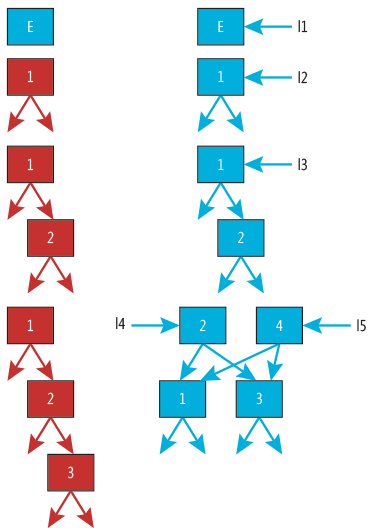
\includegraphics[width=0.4\textwidth]{lists.png}
		\end{center}
		\begin{exampleblock}{F\#}
			\begin{lstlisting}
let list3 = [3; 4]
let list1 = 2 :: list3
let list2 = 1 :: list3
            \end{lstlisting}
        \end{exampleblock}
		\begin{itemize}
			\item Списки немутабельны
			\item Cons-ячейки, указывающие друг на друга
			\item cons за константное время, @ --- за линейное
		\end{itemize}
\end{frame}

	\begin{frame}
		\frametitle{Операции над списками}
		\framesubtitle{Модуль Microsoft.FSharp.Collections.List}
		\begin{small}
			\begin{tabu} {| X[0.5 l p] | X[1 l p] | X[1 l p] | X[0.5 l p] |}
				\tabucline-
				Функция                & Описание                            & Пример                                              & Результат                        \\
				\tabucline-
				\everyrow{\tabucline-}
				List.length            & Длина списка                        & $List.length\ [1;2;3]$                              & $3$          \\
				List.nth               & n-ый элемент списка                 & $List.nth\ [1; 2; 3]\ 1$                            & $2$          \\
				List.init              & Генерирует список                   & $List.init\ 3 (fun\ i\ \rightarrow\ i * i)$         & $[0; 1; 4]$          \\
				List.head              & Голова списка                       & $List.head\ [1; 2; 3]$                              & $1$          \\
				List.tail              & Хвост списка                        & $List.tail\ [1; 2; 3]$                              & $[2; 3]$          \\
				List.map               & Применяет функцию ко всем элементам & $List.map\ (fun\ i\ \rightarrow\ i * i)\ [1; 2; 3]$ & $[1; 4; 9]$          \\
				List.filter            & Отбирает нужные элементы            & $List.filter\ (fun\ x\ \rightarrow\ x\ \%\ 2 <> 0)\ [1; 2; 3]$ & $[1; 3]$          \\
				List.fold              & "Свёртка"  & $List.fold\ (fun\ x\ acc\ \rightarrow\ acc * x)\ 1\ [1; 2; 3]$               & $6$
			\end{tabu}
		\end{small}
	\end{frame}
	
	\begin{frame}[fragile]
		\frametitle{Тип Option}
		Либо \textit{Some что-то}, либо \textit{None}, представляет возможное отсутствие значения.
		\begin{exampleblock}{F\#}
			\begin{lstlisting}
let people = [ ("Adam", None); ("Eve" , None);
    ("Cain", Some("Adam","Eve"));
    ("Abel", Some("Adam","Eve")) ]
            \end{lstlisting}
		\end{exampleblock}
		\begin{exampleblock}{F\#}
			\begin{lstlisting}
let showParents (name, parents) =
    match parents with
    | Some(dad, mum) -> 
        printfn "%s, father %s, mother %s" name dad mum
    | None -> printfn "%s has no parents!" name
            \end{lstlisting}
		\end{exampleblock}
\end{frame}

	\section{Функции}

	\begin{frame}[fragile]
		\frametitle{Рекурсия}
		\begin{exampleblock}{F\#}
			\begin{lstlisting}
let rec length l =
    match l with
    | [] -> 0
    | h :: t -> 1 + length t

let rec even n = (n = 0u) || odd(n - 1u)
and odd n = (n <> 0u) && even(n - 1u)			
            \end{lstlisting}
		\end{exampleblock}
\end{frame}

	\begin{frame}[fragile]
		\frametitle{Операторы $|>$ и $>>$}
		\framesubtitle{Forward pipeline и Композиция}
		\begin{exampleblock}{F\#}
			\begin{lstlisting}
let sumFirst3 ls = ls |> Seq.take 3 |> Seq.fold (+) 0
            \end{lstlisting}
        \end{exampleblock}
        или
		\begin{exampleblock}{F\#}
			\begin{lstlisting}
let sumFirst3 = Seq.take 3 >> Seq.fold (+) 0
            \end{lstlisting}
		\end{exampleblock}
\end{frame}

	\begin{frame}[fragile]
		\frametitle{Каррирование, частичное применение}
		\begin{exampleblock}{F\#}
			\begin{lstlisting}
let shift (dx, dy) (px, py) = (px + dx, py + dy)
let shiftRight = shift (1, 0)
let shiftUp = shift (0, 1)
let shiftLeft = shift (-1, 0)
let shiftDown = shift (0, -1)
            \end{lstlisting}
		\end{exampleblock}
		\begin{alertblock}{F\# Interactive}
			\begin{lstlisting}
> shiftDown (1, 1);;
val it : int * int = (1, 0)
            \end{lstlisting}
		\end{alertblock}
\end{frame}

	\section{.NET}

	\begin{frame}[fragile]
		\frametitle{Использование библиотек .NET}
		\begin{exampleblock}{F\#}
			\begin{lstlisting}[basicstyle=\ttfamily\tiny]
open System.Windows.Forms

let form = new Form(Visible = false, TopMost = true, Text = "Welcome to F#")
let textB = new RichTextBox(Dock = DockStyle.Fill, Text = "Some text")
form.Controls.Add(textB)

open System.IO
open System.Net

/// Get the contents of the URL via a web request
let http(url: string) =
    let req = System.Net.WebRequest.Create(url)
    let resp = req.GetResponse()
    let stream = resp.GetResponseStream()
    let reader = new StreamReader(stream)
    let html = reader.ReadToEnd()
    resp.Close()
    html

textB.Text <- http("http://www.google.com")

form.ShowDialog () |> ignore
           \end{lstlisting}
       \end{exampleblock}
\end{frame}

	\section{Сопоставление шаблонов}
	
	\begin{frame}[fragile]
		\frametitle{Сопоставление шаблонов}
\begin{exampleblock}{F\#}
\begin{lstlisting}
let urlFilter url agent =
    match (url, agent) with
    | "http://www.google.com", 99 -> true
    | "http://www.yandex.ru" , _ -> false
    | _, 86 -> true
    | _ -> false
\end{lstlisting}
\end{exampleblock}

\begin{exampleblock}{F\#}
\begin{lstlisting}
let sign x =
    match x with
    | _ when x < 0 -> -1
    | _ when x > 0 -> 1
    | _ -> 0
\end{lstlisting}
\end{exampleblock}
\end{frame}

	\begin{frame}[fragile]
		\frametitle{F\# --- не Prolog}
		Не получится писать так:
\begin{exampleblock}{F\#}
\begin{lstlisting}
let isSame pair =
    match pair with
    | (a, a) -> true
    | _ -> false
\end{lstlisting}
\end{exampleblock}
Нужно так:		
\begin{exampleblock}{F\#}
\begin{lstlisting}
let isSame pair =
    match pair with
    | (a, b) when a = b -> true
    | _ -> false
\end{lstlisting}
\end{exampleblock}
\end{frame}

	\begin{frame}
		\frametitle{Какие шаблоны бывают}
		\begin{small}
			\begin{tabu} {| X[0.9 l p] | X[1 l p] | X[1 l p] |}
				\tabucline-
				Синтаксис                               & Описание                  & Пример                                \\
				\tabucline-
				\everyrow{\tabucline-}
				$(pat, \ldots, pat)$                    & Кортеж                    & $(1, 2, (``3``, x))$                    \\
				$[pat; \ldots; pat]$                       & Список                    & $[x; y; 3]$                           \\
				$pat :: pat$                            & cons                      & $h :: t$                              \\
				$pat\ |\ pat$                             & "Или"                     & $[x]\ |\ [``X``\ |\ x]$                     \\
				$pat\ \&\ pat$                            & "И"                       & $[p] \& [(x, y)]$                     \\
				$pat\ as\ id$                             & Именованный шаблон        & $[x]\ as\ inp$                          \\
				$id$                                    & Переменная                & $x$                                   \\
				$\_$                                     & Wildcard (что угодно)     & $\_$                                   \\
				литерал                               & Константа                 & $239, DayOfWeek.Monday$ \\
				$:?\ type$                               & Проверка на тип           & $:?\ string$                           \\
			\end{tabu}
		\end{small}
	\end{frame}

	\section{Последовательности}
	
	\begin{frame}[fragile]
		\frametitle{Последовательности}
		\framesubtitle{Ленивый тип данных}
		\begin{exampleblock}{F\#}
			\begin{lstlisting}
seq {0 .. 2}
seq {1I .. 1000000000000I}
\end{lstlisting}
\end{exampleblock}

		\begin{exampleblock}{F\#}
			\begin{lstlisting}
open System.IO
let rec allFiles dir =
    Seq.append
    (dir |> Directory.GetFiles)
    (dir |> Directory.GetDirectories 
         |> Seq.map allFiles 
         |> Seq.concat)
\end{lstlisting}
\end{exampleblock}
\end{frame}

	\begin{frame}
		\frametitle{Типичные операции с последовательностями}
		\begin{small}
			\begin{tabu} {| X[0.5 l p] | X[1 l p] |}
				\tabucline-
				Операция                               & Тип                    \\
				\tabucline-
				\everyrow{\tabucline-}
				Seq.append                    & $\#seq<'a> \to \#seq<'a> \to seq<'a>$ \\
				Seq.concat                    & $\#seq<\#seq<'a>> \to seq<'a>$ \\
				Seq.choose                    & $('a \to 'b option) \to \#seq<'a> \to seq<'b>$ \\
				Seq.empty                     & $seq<'a>$ \\
				Seq.map                       & $('a \to 'b) \to \#seq<'a> \to \#seq<'b>$ \\
				Seq.filter                    & $('a \to bool) \to \#seq<'a> \to seq<'a>$ \\
				Seq.fold                      & $('s \to 'a \to 's) \to 's \to seq<'a> \to 's$ \\
				Seq.initInfinite          & $(int \to 'a) \to seq<'a>$ \\
\end{tabu}
\end{small}
\end{frame}

	\begin{frame}[fragile]
		\frametitle{Задание последовательностей}
			\begin{exampleblock}{F\#}
				\begin{lstlisting}
let squares = seq { for i in 0 .. 10 -> (i, i * i) }
seq { for (i, isquared) in squares -> 
         (i, isquared, i * isquared) }
\end{lstlisting}
\end{exampleblock}
			
			\begin{exampleblock}{F\#}
				\begin{lstlisting}
let checkerboardCoordinates n =
    seq { for row in 1 .. n do
        for col in 1 .. n do
            if (row + col) % 2 = 0 then
                yield (row, col) }
\end{lstlisting}
\end{exampleblock}	
\end{frame}

	\section{Записи}
	
	\begin{frame}[fragile]
		\frametitle{Записи}
		\begin{exampleblock}{F\#}
			\begin{lstlisting}
type Person =
    { Name: string;
      DateOfBirth: System.DateTime; }
\end{lstlisting}
\end{exampleblock}

		\begin{exampleblock}{F\#}
			\begin{lstlisting}
{ Name = "Bill"; 
  DateOfBirth = new System.DateTime(1962, 09, 02) }

{ new Person
  with Name = "Anna"
  and DateOfBirth = new System.DateTime(1968, 07, 23) }
\end{lstlisting}
\end{exampleblock}
	
\end{frame}

	\section{Размеченные объединения}
	
	\begin{frame}[fragile]
		\frametitle{Размеченные объединения}
		\framesubtitle{Discriminated unions}
		\begin{exampleblock}{F\#}
			\begin{lstlisting}
type Route = int
type Make = string
type Model = string

type Transport =
    | Car of Make * Model
    | Bicycle
    | Bus of Route
\end{lstlisting}
\end{exampleblock}
		
\end{frame}

	\begin{frame}[fragile]
		\frametitle{Известные примеры}
		\begin{exampleblock}{F\#}
			\begin{lstlisting}
type 'a option =
    | None
    | Some of 'a
\end{lstlisting}
\end{exampleblock}

		\begin{exampleblock}{F\#}
			\begin{lstlisting}
type 'a list =
    | ([])
    | (::) of 'a * 'a list
\end{lstlisting}
\end{exampleblock}
		
\end{frame}

	\begin{frame}[fragile]
		\frametitle{Использование размеченных объединений}
		\begin{exampleblock}{F\#}
			\begin{lstlisting}
type IntOrBool = I of int | B of bool
let i = I 99
let b = B true
\end{lstlisting}
\end{exampleblock}
		
		\begin{exampleblock}{F\#}
			\begin{lstlisting}
type C = Circle of int | Rectangle of int * int

[1..10]
|> List.map Circle

[1..10]
|> List.zip [21..30]
|> List.map Rectangle
\end{lstlisting}
\end{exampleblock}
		
\end{frame}

	\begin{frame}[fragile]
		\frametitle{Использование в match}
		\begin{exampleblock}{F\#}
			\begin{lstlisting}
type Tree<'a> =
    | Tree of 'a * Tree<'a> * Tree<'a>
    | Tip of 'a

let rec size tree =
    match tree with
    | Tree(_, l, r) -> 1 + size l + size r
    | Tip _ -> 1
\end{lstlisting}
\end{exampleblock}
		
\end{frame}

	\begin{frame}[fragile]
		\frametitle{Пример}
		\framesubtitle{Дерево разбора логического выражения}
		\begin{exampleblock}{F\#}
			\begin{lstlisting}
type Proposition =
    | True
    | And of Proposition * Proposition
    | Or of Proposition * Proposition
    | Not of Proposition

let rec eval (p: Proposition) =
    match p with
    | True -> true
    | And(p1, p2) -> eval p1 && eval p2
    | Or (p1, p2) -> eval p1 || eval p2
    | Not(p1) -> not (eval p1)

printfn "%A" <| eval (Or(True, And(True, Not True)))
\end{lstlisting}
\end{exampleblock}
		
\end{frame}

	\begin{frame}[fragile]
		\frametitle{Взаимосвязанные типы}
		\begin{exampleblock}{F\#}
			\begin{lstlisting}
type node =
    { Name : string;
      Links : link list }
and link =
    | Dangling
    | Link of node
\end{lstlisting}
\end{exampleblock}
		
\end{frame}

	\section{Паттерны ФП}

	\begin{frame}[fragile]
		\frametitle{Замена цикла рекурсией}
		\framesubtitle{Императивное разложение на множители}
		\begin{exampleblock}{F\#}
			\begin{lstlisting}
let factorizeImperative n =
    let mutable primefactor1 = 1
    let mutable primefactor2 = n
    let mutable i = 2
    let mutable fin = false
    while (i < n && not fin) do
        if (n % i = 0) then
            primefactor1 <- i
            primefactor2 <- n / i
            fin <- true
        i <- i + 1
    if (primefactor1 = 1) then None
    else Some (primefactor1, primefactor2)
\end{lstlisting}
\end{exampleblock}

\end{frame}

	\begin{frame}[fragile]
		\frametitle{Замена цикла рекурсией}
		\framesubtitle{Рекурсивное разложение на множители}
		\begin{exampleblock}{F\#}
			\begin{lstlisting}
let factorizeRecursive n =
    let rec find i =
        if i >= n then None
        elif (n % i = 0) then Some(i, n / i)
        else find (i + 1)
    find 2
\end{lstlisting}
\end{exampleblock}
		
\end{frame}

\begin{frame}[fragile]
	\frametitle{Хвостовая рекурсия, проблема}
	\framesubtitle{Императивный вариант}
	\begin{exampleblock}{F\#}
		\begin{lstlisting}
open System.Collections.Generic

let createMutableList() =
    let l = new List<int>()
    for i = 0 to 100000 do
        l.Add(i)
    l
\end{lstlisting}
\end{exampleblock}
	
\end{frame}

\begin{frame}[fragile]
	\frametitle{Хвостовая рекурсия, проблема}
	\framesubtitle{Рекурсивный вариант, казалось бы}
	\begin{exampleblock}{F\#}
		\begin{lstlisting}
let createImmutableList() =
    let rec createList i max =
        if i = max then
            []	
        else
            i :: createList (i + 1) max
    createList 0 100000
\end{lstlisting}
\end{exampleblock}
	
\end{frame}

\begin{frame}[fragile]
	\frametitle{Факториал без хвостовой рекурсии}
	\begin{exampleblock}{F\#}
		\begin{lstlisting}
let rec factorial x =
    if x <= 1
    then 1 
    else x * factorial (x - 1)
\end{lstlisting}
\end{exampleblock}
	
	\begin{exampleblock}{F\#}
		\begin{lstlisting}
let rec factorial x =
    if x <= 1
    then
        1
    else
        let resultOfRecusion = factorial (x - 1)
        let result = x * resultOfRecusion
        result
\end{lstlisting}
\end{exampleblock}
	
\end{frame}

\begin{frame}[fragile]
	\frametitle{Факториал с хвостовой рекурсией}
	\begin{exampleblock}{F\#}
		\begin{lstlisting}
let factorial x =
    let rec tailRecursiveFactorial x acc =
        if x <= 1 then
            acc
        else
            tailRecursiveFactorial (x - 1) (acc * x)
    tailRecursiveFactorial x 1
\end{lstlisting}
\end{exampleblock}

\end{frame}
	
\begin{frame}[fragile]
	\frametitle{После декомпиляции в C\#}
		\begin{alertblock}{C\#}
			\begin{lstlisting}[language=Java]
public static int tailRecursiveFactorial(int x, int acc)
{
    while (true)
    {
        if (x <= 1)
        {
            return acc;
        }
        acc *= x;
        x--;
    }
}
\end{lstlisting}
\end{alertblock}
	
\end{frame}

\begin{frame}[fragile]
	\frametitle{Паттерн ``Аккумулятор''}
	\begin{exampleblock}{F\#}
		\begin{lstlisting}
let rec map f list =
    match list with
    | [] -> []
    | hd :: tl -> (f hd) :: (map f tl)

let map f list =
    let rec mapTR f list acc =
        match list with
        | [] -> acc
        | hd :: tl -> mapTR f tl (f hd :: acc)
    mapTR f (List.rev list) []
\end{lstlisting}
\end{exampleblock}
	
\end{frame}

\begin{frame}[fragile]
	\frametitle{Continuation Passing Style}
	\frametitle{Аккумулятор --- функция}
	\begin{exampleblock}{F\#}
		\begin{lstlisting}
let printListRev list =
    let rec printListRevTR list cont =
        match list with
        | [] -> cont ()
        | hd :: tl ->
            printListRevTR tl (fun () -> 
                printf "%d " hd; cont () )
    printListRevTR list (fun () -> printfn "Done!")
\end{lstlisting}
\end{exampleblock}
	
\end{frame}

\end{document}



